% SAIV 2026 Submission - LNCS Format (Springer Lecture Notes in Computer Science)
% Adapted from ICML 2026 draft
\documentclass[runningheads]{llncs}

\usepackage[T1]{fontenc}
\usepackage{amsmath}
\usepackage{amsfonts}
\usepackage{amssymb}
\usepackage{graphicx}
\usepackage{booktabs}
\usepackage{hyperref}
\usepackage{array}
\usepackage{multirow}
\usepackage{float}
\usepackage{xcolor}
\usepackage{bbm}
\usepackage{algorithm}
\usepackage{algpseudocode}
\usepackage{microtype}
\usepackage{pgfplots}
\usepackage{pgfplotstable}
\pgfplotsset{compat=1.18}
\usetikzlibrary{patterns,positioning,arrows.meta,calc}


%%%%% FOR STRIKETHROUGH %%%%%
\usepackage[normalem]{ulem}
\newcommand{\BW}[1]{{\color{red} #1}}
\newcommand{\redsout}[1]{{\color{red}\sout{{\color{black}#1}}}}

\begin{document}

\title{{\textsf{MetaMoE}:} Formal Verification of Compositional Robustness and Scalability of Mixture-of-Experts Architecture}
\titlerunning{Compositional Robustness of Mixture-of-Experts}

\author{Quang Pham \and Ben Wooding \and Luke Nam \and Samuel Sasaki \and Taylor T. Johnson}
\authorrunning{Q. Pham et al.}

\institute{Institute for Software Integrated Systems, Vanderbilt University, Nashville, TN, USA\\
\email{\{quang.m.pham, ben.wooding, luke.nam, samuel.sasaki, taylor.johnson\}@vanderbilt.edu}}
\maketitle

\begin{abstract}
Mixture-of-experts (MoE) architectures offer modularity and scalability, yet their robustness, and the practicality of certifying that robustness, in heterogeneous settings are not well understood. This work presents \textsf{MetaMoE}, a heterogeneous MoE framework designed for compositional formal verification. In \textsf{MetaMoE}, a neural network, called a router, classifies an input image's domain and routes it to the corresponding domain expert neural network for fine-grained classification; we study how robustness propagates compositionally across these router and experts and establish when system-level verification can be derived from component-level verification. In homogeneous MoE, all experts share the same task, so a misroute may still preserve correctness if the receiving expert classifies the input correctly; in heterogeneous MoE, experts operate on disjoint class spaces, making any misroute catastrophic. We prove that when the router maintains expert selection within a perturbation limit, and the selected expert also maintains its classification within that perturbation limit, the end-to-end system robustness is compositional. This enables scalability as the computational power needed for verification and re-verification does not snowball as the system expands. We further validate the formal certified robustness results with empirical adversarial testing. Experiments across 8 MoE configurations and 3 perturbation budgets show that robustly trained (RT) experts improve adversarial accuracy by up to $13.1\%$ over non-robustly trained (NRT) ones and are a prerequisite for formal certifiability -- NRT models on complex domains are completely unverifiable -- while router training paradigm has negligible impact ($<0.1\%$), and verified routers achieve $100\%$ certified robustness accuracy (RoCRA) at practical perturbation bounds. These results outline a principled path toward scalable, verifiable modular AI. 

\keywords{Mixture-of-experts \and Adversarial Robustness \and Formal Verification \and Compositional Verification \and Neural Network Verification \and Safety-Critical AI}
\end{abstract}

\section{Introduction}

Deep neural networks (DNNs) achieve high accuracy on image classification tasks but remain vulnerable to small adversarial perturbations~\cite{goodfellow2015,madry2018}. This unreliability is hard to justify in safety-critical vision applications such as autonomous driving, traffic-sign recognition, and medical imaging. In parallel, Mixture-of-experts (MoE) architectures~\cite{jacobs1991,shazeer2017}, originally proposed in the early 1990s and recently revitalized for large-scale deep learning, offer a powerful paradigm for scaling models through modular computation and conditional activation. The core idea is to replace a single monolithic neural network with a collection of smaller, specialized sub-networks called \emph{experts}, each is trained to handle a specific subset of input space, together with a neural network \emph{router} that examines each input and decides which expert(s) should process it. Since only one or a few experts are activated per input, MoE systems' computation and inference costs increase slower than system capacity. While recent work has popularized MoE primarily within large language models~\cite{shazeer2017,deepseek2024}, the paradigm is equally viable for \emph{vision} systems~\cite{riquelme2021} where distinct visual domains (\emph{e.g.}, traffic signs~\cite{gtsrb}, handwritten digits~\cite{mnist1998}, \emph{etc.}) benefit from dedicated expert networks. Yet the robustness properties of such heterogeneous vision MoE systems, where domain-specific experts must cooperate under a shared router, remain poorly understood.

Formal verification tools such as $\alpha$--$\beta$-CROWN~\cite{wang2021} can certify provable robustness for individual neural networks, yet verifying a full MoE system remains challenging because the verifier must reason jointly about the router, every expert, and their interactions. This raises a natural question: can the verified robustness of individual experts and the router be combined to certify the full system? An affirmative answer would allow heterogeneous MoE systems to be trained, extended with new experts, and certified modularly, avoiding the need to re-verify the entire system whenever a single component changes.

This paper introduces \textsf{MetaMoE}, a verification-aware heterogeneous MoE architecture in which each input carries two labels: a fine-grained \emph{class} (\emph{e.g.}, speed-limit sign) and a coarse \emph{meta-class} identifying the domain (\emph{e.g.}, German traffic signs vs.\ handwritten digits). The router learns to predict the meta-class and dispatches the input to the corresponding domain expert, which then predicts the fine-grained class. This two-level classification motivates the name \emph{Meta}MoE (Figure~\ref{fig:metamoe-arch}). The framework combines verifiable experts with a verifiable routing network, intermixing adversarially and non-adversarially trained components. We investigate how empirical adversarial robustness, measured by accuracy under Projected Gradient Descent (PGD) attacks~\cite{madry2018}, where higher accuracy indicates greater resilience to worst-case perturbations, relates to certified robustness (formal bounds), and establish conditions under which these guarantees propagate from individual components to the entire system.

\begin{figure}[t]
\centering
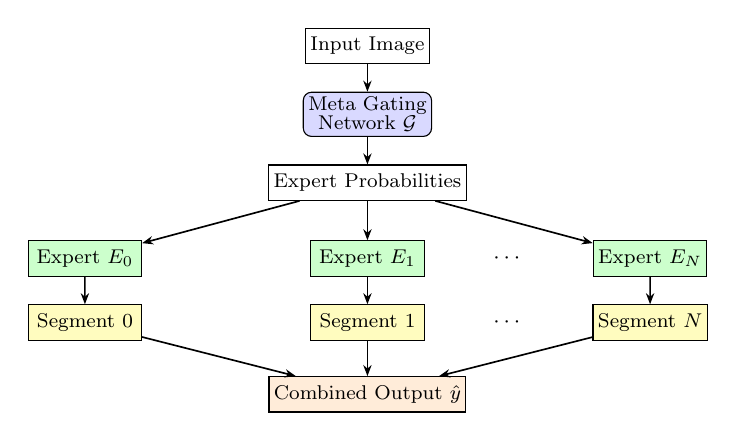
\begin{tikzpicture}[scale=0.9, every node/.style={scale=0.9},
    node distance=0.35cm and 0.45cm,
    box/.style={draw, rectangle, minimum width=1.6cm, minimum height=0.5cm, align=center, font=\footnotesize, inner sep=2pt},
    routerbox/.style={box, fill=blue!15, rounded corners=3pt},
    expertbox/.style={box, fill=green!20},
    segbox/.style={box, fill=yellow!25},
    outbox/.style={box, fill=orange!15, minimum width=2.4cm},
    arr/.style={-{Stealth[length=4pt]}, semithick},
]
% Input
\node[box] (input) {Input Image};

% Router
\node[routerbox, below=of input] (router) {Meta Gating\\[-2pt]Network $\mathcal{G}$};

% Expert Probabilities
\node[box, below=of router] (probs) {Expert Probabilities};

% Experts row
\node[expertbox, below left=0.5cm and 1.6cm of probs] (e0) {Expert $E_0$};
\node[expertbox, below=0.5cm of probs] (e1) {Expert $E_1$};
\node[expertbox, below right=0.5cm and 1.6cm of probs] (en) {Expert $E_N$};
\node[font=\small] at ($(e1)!0.5!(en)$) {$\cdots$};

% Segment row
\node[segbox, below=0.35cm of e0] (s0) {Segment 0};
\node[segbox, below=0.35cm of e1] (s1) {Segment 1};
\node[segbox, below=0.35cm of en] (sn) {Segment $N$};
\node[font=\small] at ($(s1)!0.5!(sn)$) {$\cdots$};

% Combined Output
\node[outbox, below=0.45cm of s1] (output) {Combined Output $\hat{y}$};

% Arrows
\draw[arr] (input) -- (router);
\draw[arr] (router) -- (probs);
\draw[arr] (probs) -- (e0);
\draw[arr] (probs) -- (e1);
\draw[arr] (probs) -- (en);
\draw[arr] (e0) -- (s0);
\draw[arr] (e1) -- (s1);
\draw[arr] (en) -- (sn);
\draw[arr] (s0) -- (output);
\draw[arr] (s1) -- (output);
\draw[arr] (sn) -- (output);
\end{tikzpicture}
\caption{\textsf{MetaMoE} architecture. The meta gating network $\mathcal{G}$ receives the input image and produces routing probabilities over $N$ experts. Under hard routing ($k{=}1$), the top-scoring expert $E_{m^*}$ is activated; its output populates the corresponding segment of the unified output vector $\hat{y} \in \mathbb{R}^{C_{\text{total}}}$ (Eq.~1), with all other segments zeroed. Experts are frozen after independent training; only $\mathcal{G}$ is trained during MoE composition.}
\label{fig:metamoe-arch}
\end{figure}

The central challenge is that verifying an MoE system monolithically is expensive: the verifier must reason about the router, all experts, and their interactions simultaneously. Our key insight is that under hard routing, exactly one expert processes each input, so the system decomposes naturally into two independent verification tasks: does the router select the right expert?, and does that expert classify correctly? If both hold, the system is correct. This insight leads to three contributions, each building on the previous:

\begin{enumerate}
    \item \textbf{Compositional Robustness (Theorem~\ref{thm:compositional}).} We prove an assume-guarantee rule for hard-routed MoE with disjoint expert class spaces: the system is robust at an input if and only if (i) the router maintains invariant expert selection within the $\ell_\infty$ perturbation ball and (ii) the selected expert is robust within that same ball. The biconditional guarantees that no interaction effects between router and expert can invalidate component-level certificates, reducing system-level verification to independent tasks whose cost is fixed regardless of how many experts the system contains.

    \item \textbf{Verification methodology.} We leverage the theorem in a practical compositional verification pipeline using $\alpha$--$\beta$-CROWN, a state-of-the-art neural network verifier. Because the theorem guarantees soundness of independent component verification, we extract the router as a standalone network and verify it separately from the experts. We describe the architecture and export decisions (BatchNorm elimination, raw logit output, and property negation for counterexample search) that make each component amenable to bound propagation. This reduces the verification target from the full system (${\sim}$231K parameters) to the largest single component (${\sim}$96K), with the reduction ratio scaling linearly with the number of experts.

    \item \textbf{Empirical case study.} We validate the theorem and methodology across 8 MoE configurations (40 training runs), 3 perturbation budgets ($\varepsilon = 2/255, 4/255, 8/255$), and 4 expert/router training combinations on CIFAR-10~\cite{cifar10}, MNIST~\cite{mnist1998}, GTSRB~\cite{gtsrb}, and PTSD~\cite{ptsd}. The case study reveals three practical findings: (i) for visually dissimilar domains, expert robustness dominates system behavior while router adversarial training has negligible impact ($< 0.1\%$ accuracy difference), meaning the router can be trained without costly adversarial augmentation; (ii) within each domain and architecture, higher empirical adversarial accuracy (AA) monotonically associates with higher expert certified robustness (ExCRA), providing a cheap proxy for formal verifiability; and (iii) robust training is a prerequisite for verifiability; non-robustly trained models on complex domains are completely unverifiable.
\end{enumerate}

\section{Related Work}

Sparse gating~\cite{shazeer2017} made MoE~\cite{jacobs1991} practical at scale, and subsequent work extended the paradigm to vision~\cite{riquelme2021}, demonstrated that freezing pretrained experts reduces retraining cost for lifelong learning~\cite{fedus2022}, and scaled sparse routing to hundreds of billions of parameters~\cite{dai2024,jiang2024,deepseek2024}. Complementary advances in catastrophic-forgetting mitigation~\cite{ramasesh2022}, gating evolution from unsupervised~\cite{jordan1994} to supervised~\cite{riquelme2021} schemes, and modular deep learning~\cite{pfeiffer2023} have established MoE as a mature paradigm for composable model design.

Yet this scalability work largely ignores a critical question: \emph{are MoE systems robust, and can that robustness be formally certified?} The few studies that examine MoE robustness each address a different facet of this question without resolving it holistically. Puigcerver et al.~\cite{puigcerver2022} showed that sparse MoE Vision Transformers can be more robust than dense counterparts at the same computation cost, but their formal guarantees are derived only for simplified settings with smooth MoEs or linear experts under fixed routing and structured data-separation assumptions. Zhang et al.~\cite{zhang2025moe} studied model-level MoE ensembles of identical experts and found that \emph{within} such systems, the expert networks are the primary vulnerability (far more susceptible to adversarial attack than the router), a complementary rather than contradictory finding since it characterizes where vulnerability concentrates rather than whether MoE improves overall robustness. Pavlitska et al.~\cite{pavlitska2025robust} confirmed that sparse MoE layers inside CNNs improve adversarial robustness when combined with adversarial training, though MoE structure alone confers negligible benefit. All three studies examine \emph{homogeneous} MoE (same experts, same dataset); none consider \emph{heterogeneous} MoE with disjoint expert domains, nor do they analyze how robustness propagates through the router-expert composition or connect empirical resilience to provable certificates.

Meanwhile, neural network verification has matured as an independent line of research. Katz et al.~\cite{katz2017} established the NP-completeness of the general problem, and Alsmann and Lange~\cite{alsmann2025complexity} recently extended complexity analysis to state space models, showing that satisfiability is undecidable in the general case and NP-complete under bounded context. These hardness results motivate scalable approximations: $\alpha$--$\beta$-CROWN~\cite{wang2021} provides state-of-the-art complete verification via bound propagation (current winner of VNN-COMP~\cite{kaulen2025}), NNV~\cite{tran2020nnv} offers reachability-based verification for cyber-physical systems, and GRENA~\cite{zhong2025grena} scales abstract refinement to CNNs via GPU-accelerated unconstrained optimization. Certified training methods such as CROWN-IBP~\cite{zhang2020} and randomized smoothing~\cite{cohen2019} produce models with built-in provable guarantees, while the robustness margin~\cite{kielhoefer2025robustness} characterizes robustness independently of a fixed $\varepsilon$. PGD-based adversarial training~\cite{madry2018} provides complementary empirical robustness, and probabilistic verification~\cite{chwialkowski2025probabilistic} bridges the gap between formal and statistical guarantees. However, all of these tools and techniques target \emph{monolithic} networks; they cannot directly certify a system whose behavior depends on dynamic routing among multiple sub-networks.

One promising solution is compositional verification, long established in classical systems through assume-guarantee reasoning~\cite{henzinger1998}. Zhou and Tripakis~\cite{zhou2024compositional} recently adapted compositional inductive invariants to neural network controlled systems, demonstrating that modular proofs can scale where monolithic analysis cannot. Watson et al.~\cite{watson2025scenario} decompose verification of autonomous perception systems into environment-specific scenarios with composed probabilistic guarantees. However, both frameworks address feedback control loops or perception pipelines, not the conditional-activation structure of MoE, where a router's decision determines which expert's guarantees apply.

These three lines of work (MoE scalability, adversarial robustness, and formal verification) have developed largely in isolation. MoE research scales models without certifying them; robustness studies attack or defend MoE empirically without formal guarantees; and verification certifies monolithic networks without addressing compositional, dynamically-routed architectures. This paper bridges all three by asking: \textit{Can compositional robustness in heterogeneous MoE systems be formally verified and empirically validated?} We answer affirmatively by proving that router invariance and expert robustness compose to yield system-level guarantees, and by showing that empirical adversarial accuracy correlates with formal certifiability in our study.

\section{Problem Formulation}

We define the following notation used throughout this paper. Let $x \in \mathbb{R}^{C \times H \times W}$ denote a normalized input image, where $C = 3$ is the number of color channels (RGB), $H$ is the image height, and $W$ is the image width (in our experiments, $H = W = 32$ pixels). Let $N$ denote the total number of domain-specific experts in the system, and let $C_i$ denote the number of classes in dataset~$i$ (\emph{e.g.}, $C_i = 10$ for CIFAR-10, $C_i = 43$ for GTSRB). The total number of classes across all datasets is $C_{\text{total}} = \sum_{i=1}^{N} C_i$, and the target class label is $y \in \{1, \ldots, C_{\text{total}}\}$.

A heterogeneous MoE system consists of two types of components:

\begin{enumerate}
    \item \textbf{Experts:} Each expert $E_i$ is a neural network specialized for dataset~$i$. It maps an input image to a vector of class logits (unnormalized scores) for its domain: $E_i: \mathbb{R}^{C \times H \times W} \to \mathbb{R}^{C_i}$, producing $y_i = E_i(x)$ where $y_i \in \mathbb{R}^{C_i}$ is the logit vector for domain~$i$.
    \item \textbf{Router:} The router (also called gating network) $\mathcal{G}$ determines which expert should handle a given input. It maps the input image to $N$ routing logits: $\mathcal{G}: \mathbb{R}^{C \times H \times W} \to \mathbb{R}^N$, producing $g = \mathcal{G}(x)$ where $g_i$ is the routing score for expert~$i$.
\end{enumerate}

Under hard routing (top-1 selection), the router selects a single expert $m^* = \arg\max_i g_i$, i.e., the expert with the highest routing score. For top\nobreakdash-$k$ routing (where $k$ experts are activated simultaneously), let $\mathcal{S} = \{s_1, \ldots, s_k\} \subset \{1, \ldots, N\}$ denote the indices of the $k$ experts with the highest routing scores. Each selected expert~$s_j$ receives a normalized weight:
\begin{equation*}
    w_j = \frac{g_{s_j}}{\sum_{\ell=1}^{k} g_{s_\ell}}, \quad j = 1, \ldots, k
\end{equation*}
representing its contribution to the final output. To combine outputs from experts with different class spaces, we define \emph{class offsets} $o_i = \sum_{m<i} C_m$ so that expert~$i$'s classes occupy positions $o_i$ through $o_i + C_i - 1$ in a unified output vector $\hat{y} \in \mathbb{R}^{C_{\text{total}}}$. The unified MoE output $\hat{y}$ (distinct from the target label~$y$) is:
\begin{equation}
\label{eq:first}
    \hat{y}_c = \begin{cases}
        w_j \cdot y_{s_j}[c - o_{s_j}], & \text{if } c \in \{o_{s_j}, \ldots, o_{s_j} + C_{s_j} - 1\} \text{ for some } j \in \{1, \ldots, k\} \\
        0, & \text{otherwise}
    \end{cases}
\end{equation}
where $\hat{y}_c$ is the $c$-th element of the unified output and $y_{s_j}[c - o_{s_j}]$ retrieves the logit from expert~$s_j$ at local class index $c - o_{s_j}$.

\subsection{Adversarial Threat Model and Robustness}
\label{sec:threat-model}

We consider an adversary that applies a small perturbation $\delta \in \mathbb{R}^{C \times H \times W}$ to the input, bounded under the $\ell_\infty$ norm: $\|\delta\|_\infty \leq \varepsilon$, where $\varepsilon > 0$ is the perturbation budget (\emph{e.g.}, $\varepsilon = 8/255 \approx 0.031$ in pixel intensity). This produces adversarial examples $x' = x + \delta$ lying within the $\varepsilon$-ball $B_\varepsilon(x) = \{x' : \|x' - x\|_\infty \leq \varepsilon\}$, i.e., the set of all images within $\varepsilon$ of the original input in every pixel channel. Robustness requires that the model's prediction remains correct for \emph{all} perturbations within this ball:

\begin{itemize}
    \item \textbf{Expert $E_i$ robustness:} Given that the router has already selected expert~$i$, the expert itself must still predict the correct class even when the input is slightly perturbed. Formally, the expert's predicted class is unchanged: $\arg\max_c\, y_i(x')[c] = y$ for all $x' \in B_\varepsilon(x)$, where $y_i(x') = E_i(x')$ is the logit vector of expert~$i$ on the perturbed input. In other words, no small perturbation can cause the expert to misclassify the input within its own task domain.
    \item \textbf{Router $\mathcal{G}$ robustness (invariance):} The router must consistently delegate the input to the same expert regardless of small perturbations, ensuring that an adversary cannot trick the system into activating the wrong expert. Formally, $m^*(x') = m^*(x)$ for all $x' \in B_\varepsilon(x)$, meaning the router's expert selection is invariant within the $\varepsilon$-ball. Equivalently, the selected expert's routing logit remains strictly dominant over all alternatives: $g_{m^*}(x') - g_j(x') > 0$ for all $j \neq m^*$ and all $x' \in B_\varepsilon(x)$.
    \item \textbf{MoE system robustness:} The end-to-end system -- comprising both the router and the selected expert -- must produce the correct final classification under perturbation. This is the strongest requirement, as it demands that neither the routing decision nor the expert's prediction is corrupted. Formally, $\arg\max_c \hat{y}_c(x') = y$ for all $x' \in B_\varepsilon(x)$, where $\hat{y}(x')$ is the unified MoE output~\eqref{eq:first}.
\end{itemize}

We quantify verifiability with two \emph{certified} metrics, each computed by a formal verifier over a finite test set~$D$. For a single test image $(x,y)$, the verifier returns a binary verdict: either it \emph{proves} that the property holds for every perturbation in $B_\varepsilon(x)$, or it cannot (timeout or counterexample). The aggregate metric is the fraction of images in~$D$ that receive a positive verdict.

\textbf{Expert Certified Robustness Accuracy (ExCRA).} For an expert $E_i$, the per-image property is correct classification under all perturbations: $\arg\max_c E_{i,c}(x') = y$ for all $x' \in B_\varepsilon(x)$. The aggregate metric is:
\begin{equation}
    \text{ExCRA}(\varepsilon) = \frac{1}{|D|} \sum_{(x,y) \in D} \mathbbm{1}\bigl[\text{Verify}(E_i, x, \varepsilon)\bigr]
\end{equation}

\textbf{Router Certified Robustness Accuracy (RoCRA).} For the router $\mathcal{G}$, the per-image property is invariant expert selection: $\arg\max_i \mathcal{G}_i(x') = m^*$ for all $x' \in B_\varepsilon(x)$, where $m^* = \arg\max_i \mathcal{G}_i(x)$. The aggregate metric is:
\begin{equation}
    \text{RoCRA}(\varepsilon) = \frac{1}{|D|} \sum_{(x,m^*) \in D} \mathbbm{1}\bigl[\text{Verify}(\mathcal{G}, x, \varepsilon)\bigr]
\end{equation}

In both cases, $\mathbbm{1}[\text{Verify}(\cdot)]$ equals~1 only when the verifier produces a formal proof; timeouts and counterexamples both yield~0. Because these metrics aggregate binary formal verdicts over a test set, a reported value such as ``ExCRA $= 90\%$'' means ``the verifier formally certified 18 out of 20 test images.''\!

\subsection{Problem Statement}

Given $N$ pretrained experts $\{E_i\}$, router $\mathcal{G}$, and $L_\infty$ adversary with radius $\varepsilon$, we investigate:
\begin{enumerate}
    \item \textbf{Compositional Robustness:} Does robust training of components yield provably robust MoE composition?
    \item \textbf{Empirical--Formal Correlation:} \BW{first introduction, I think using different terminology would be helpful. I think we should come up with a different phrase.} Does PGD AA predict ExCRA?
    \item \textbf{Scalability:} Can modular robustness achieve reduced retraining time, linear inference $O(k)$, and stable verification?
\end{enumerate}

\subsection{Compositional Robustness Theorem}
\label{sec:compositional}

Rather than verifying the MoE as a monolithic whole, we adopt assume-guarantee reasoning~\cite{henzinger1998}, in which each component \emph{assumes} certain environmental conditions and \emph{guarantees} a local property. In our setting, the router guarantees stable expert selection and each expert guarantees correct classification within its domain. We formalize this decomposition below through a definition, two supporting lemmas, and a composing theorem showing that these component-level guarantees are individually necessary and jointly sufficient for system robustness.

\begin{definition}[Router Invariance]
\label{def:router_invariance}
Router $\mathcal{G}$ is \emph{invariant} at input $x$ within perturbation ball $B_\varepsilon(x)$ if, for every perturbed input $x' \in B_\varepsilon(x)$,
\[
    \arg\max_i \mathcal{G}_i(x') = \arg\max_i \mathcal{G}_i(x).
\]
That is, no perturbation within the $\varepsilon$-ball can cause the router to select a different expert.
\end{definition}

With this definition, we establish the compositional robustness result in two steps: Lemma~\ref{lem:router} shows that router invariance fixes the active expert throughout the perturbation ball, and Lemma~\ref{lem:expert} shows that expert robustness then preserves the final classification. Theorem~\ref{thm:compositional} composes both into a biconditional.

\begin{lemma}[Router Invariance Preserves Expert Selection]
\label{lem:router}
Let $m^* = \arg\max_i \mathcal{G}_i(x)$ be the expert selected for clean input~$x$. If $\mathcal{G}$ is invariant at $x$ within $B_\varepsilon(x)$ (Definition~\ref{def:router_invariance}), then $m^*(x') = m^*$ for all $x' \in B_\varepsilon(x)$, and the MoE output reduces to a fixed expert's output: $\hat{y}(x') = E_{m^*}(x')$ (up to class offsets) for all $x' \in B_\varepsilon(x)$.
\end{lemma}

\begin{proof}
By Definition~\ref{def:router_invariance}, $\arg\max_i \mathcal{G}_i(x') = m^*$ for all $x' \in B_\varepsilon(x)$. Under hard routing ($k{=}1$), only expert~$m^*$ is activated, so $\hat{y}_c(x') = E_{m^*}(x')[c - o_{m^*}]$ for $c \in \{o_{m^*}, \ldots, o_{m^*} + C_{m^*} - 1\}$ and $\hat{y}_c(x') = 0$ otherwise. The MoE output is therefore fully determined by $E_{m^*}$. \qed
\end{proof}

Lemma~\ref{lem:router} eliminates the routing dimension of the problem: under hard routing, an invariant router selects the same expert for every input in the perturbation ball, so the full MoE output depends only on that expert. The remaining question is whether that expert classifies correctly throughout the ball.

\begin{lemma}[Expert Robustness Preserves Classification]
\label{lem:expert}
If expert $E_{m^*}$ is robust at $x$ within $B_\varepsilon(x)$, i.e.,
\[
    \arg\max_c\, E_{m^*,c}(x') = y \quad \text{for all } x' \in B_\varepsilon(x),
\]
and the MoE output is determined solely by $E_{m^*}$, then $\arg\max_c \hat{y}_c(x') = y$ for all $x' \in B_\varepsilon(x)$.
\end{lemma}

\begin{proof}
Since the MoE output vector $\hat{y}(x')$ is zero outside the class range of $E_{m^*}$ and equals $E_{m^*}(x')$ within that range (by Lemma~\ref{lem:router}), the argmax of $\hat{y}(x')$ coincides with the argmax of $E_{m^*}(x')$ (shifted by offset $o_{m^*}$). By assumption, this argmax equals $y$ for all $x' \in B_\varepsilon(x)$. \qed
\end{proof}

Lemma~\ref{lem:expert} completes the reduction: once routing is fixed, the unified output vector contains nonzero logits only from the selected expert, so expert-level correctness results in system-level correctness.

\begin{theorem}[Compositional Robustness]
\label{thm:compositional}
Consider a hard-routed MoE ($k{=}1$) with router $\mathcal{G}$ and experts $\{E_i\}$ having disjoint class spaces. Let $m^* = \arg\max_i \mathcal{G}_i(x)$ denote the selected expert for input~$x$. The MoE system is robust at $x$ within $B_\varepsilon(x)$ if and only if:
\begin{enumerate}
    \item[(i)] $\mathcal{G}$ is invariant at $x$ within $B_\varepsilon(x)$ (Lemma~\ref{lem:router}), and
    \item[(ii)] $E_{m^*}$ is robust at $x$ within $B_\varepsilon(x)$ (Lemma~\ref{lem:expert}).
\end{enumerate}
That is, for disjoint expert class spaces, where $m^*$ is the router-selected expert:
\begin{equation}
    \text{MoE robust at } x \;\Longleftrightarrow\; \underbrace{\text{Router invariant at } x}_{\text{same expert } m^* \text{ selected}} \;\land\; \underbrace{\text{Expert } E_{m^*} \text{ robust at } x}_{\text{correct class predicted}}
\end{equation}
\end{theorem}

\begin{proof}
\textbf{(Sufficiency.)} Follows directly by composing Lemmas~\ref{lem:router} and~\ref{lem:expert}: router invariance ensures the same expert~$m^*$ is selected for all $x' \in B_\varepsilon(x)$, and expert robustness ensures that expert produces the correct output throughout.

\textbf{(Necessity, under disjoint classes.)} Suppose condition~(i) fails: there exists $x' \in B_\varepsilon(x)$ with $m^*(x') = m' \neq m^*$. Since experts have disjoint class spaces, $E_{m'}$ outputs logits only over $m'$'s classes. Because robustness requires correct classification on all inputs in $B_\varepsilon(x)$, including the clean input~$x$ itself, and the clean system correctly classifies $x$, the true label $y$ must lie in $m^*$'s class range. Therefore $\arg\max_c \hat{y}_c(x') \neq y$, and the MoE is not robust. Now suppose (i)~holds but (ii)~fails: there exists $x' \in B_\varepsilon(x)$ with $\arg\max_c E_{m^*,c}(x') \neq y$. By Lemma~\ref{lem:router}, $\hat{y}(x')$ is determined by $E_{m^*}(x')$, so $\arg\max_c \hat{y}_c(x') \neq y$, and again the MoE is not robust. \qed
\end{proof}

The practical consequence of this assume-guarantee decomposition is \emph{modular verification}: verify router invariance and expert robustness independently, then compose guarantees via Theorem~\ref{thm:compositional}. This avoids verifying the full MoE as a monolithic network, reducing verification cost and enabling incremental certification -- when a new expert is added, only the new expert and the updated router require (re-)verification, while existing expert certificates remain valid. Note that the biconditional holds under hard routing with disjoint class spaces; for overlapping classes only sufficiency holds, and soft/top-$k$ routing requires additional invariance conditions (Section~\ref{sec:limitations}) \BW{It's always advised that you avoid forward references}. We examine the harder case of visually similar datasets (GTSRB~\cite{gtsrb} vs.\ PTSD~\cite{ptsd}) in Appendix~\ref{app:similarity} \BW{Should link to the first appendix not appedix I.This is also only one paragraph in that appendix so probably better to either expand it out or just remove it.}.

\subsection{Empirical--Formal Correlation \BW{choose a different phrase.}}

Two complementary metrics quantify robustness at different levels of rigour. \emph{Adversarial accuracy} $\text{AA}(\varepsilon)$ is an \textbf{empirical heuristic}: it measures the fraction of test images correctly classified after a PGD attack~\cite{madry2018} with budget~$\varepsilon$. Because PGD is a first-order attack that searches for (but does not guarantee finding) the worst-case perturbation, AA provides only a \emph{lower bound} on true robustness -- a model may appear robust under PGD yet be vulnerable to stronger attacks. In contrast, \emph{Expert Certified Robustness Accuracy} $\text{ExCRA}(\varepsilon)$ is a \textbf{formal metric}: it counts the fraction of test images for which a sound verifier \emph{proves} that no perturbation within $B_\varepsilon(x)$ can change the prediction (Section~\ref{sec:threat-model}). At a fixed~$\varepsilon$, soundness guarantees $\text{ExCRA} \leq \text{AA}$, since every certified image is truly robust while PGD may miss adversarial examples.

Both metrics aggregate over a test set: ``AA $= 17\%$'' means PGD found successful attacks on 83\% of test images, and ``ExCRA $= 90\%$'' means the verifier formally certified 18 out of 20 images. Neither metric is per-image in the reported percentages, though each is computed from a per-image binary outcome.

Prior work has established that adversarial training generally improves certified robustness~\cite{salman2019provably,balunovic2020adversarial}, and surveys confirm this trend across verification methods~\cite{li2023sok}. Building on this foundation, we investigate whether, within a given domain and architecture, higher AA monotonically associates with higher ExCRA, with robust training as a prerequisite for verifiability. Our experiments confirm this monotonic association and further reveal that non-robust training on complex domains yields complete verification failure (ExCRA $= 0\%$), a finding we believe to be novel.

\section{Methodology}

Given an RGB input image $x \in \mathbb{R}^{C \times H \times W}$ and $N$ domain-specific datasets each containing $C_i$ classes, we independently train $N$ expert networks $E_i: \mathbb{R}^{C \times H \times W} \to \mathbb{R}^{C_i}$ (one per dataset, frozen after training) and a single router $\mathcal{G}: \mathbb{R}^{C \times H \times W} \to \mathbb{R}^N$ that outputs one routing logit per expert. We evaluate on 7 datasets: CIFAR-10, MNIST, GTSRB~\cite{gtsrb} (diverse domains) and PTSD~\cite{ptsd}, BTSD, ETSD, TSRD (similar traffic sign domains for lifelong learning). \BW{Provide some intuition about what each of these are.}

Each expert $E_i$ is denoted $E_{i\_\text{CNN\_NRT}}$ (non-robust) \BW{too much subscript, remove the $\_CNN\_$} parts) or $E_{i\_\text{CNN\_RT}}$ (robust), where the index $i$ corresponds to: CIFAR-10 ($E_0$), MNIST ($E_1$), GTSRB ($E_2$), PTSD ($E_3$), BTSD ($E_4$), ETSD ($E_5$), TSRD ($E_6$). Full notation is provided in Appendix~\ref{app:notation}. \BW{I think its clear without needing to refer to the appendix.}

\subsection{Verification-Aware CNN Architecture}

Both experts and router use a convolutional architecture (VerifiableCNN) designed for compatibility with $\alpha$--$\beta$-CROWN's bound propagation. The architecture comprises 4 convolutional layers with gradual channel growth ($20 \to 28 \to 40 \to 56$), $2{\times}2$ average pooling in blocks 1--3, and a 2-layer fully connected head (detailed specifications in Appendix~\ref{app:architecture} \BW{(refer to appendices in order)}). Three design choices make the network amenable to LP-based verification: average pooling replaces max pooling to preserve linearity, increased channel capacity compensates for narrow widths, and static shapes minimize ONNX operators. Experts include BatchNorm (${\sim}$96K params for 43 classes), which we fold into convolutional weights during ONNX export (Appendix~\ref{app:onnx}) to eliminate BatchNorm operators from the verification graph. The router omits BatchNorm entirely for deterministic verification behavior (${\sim}$38K params). \BW{What happened to the formal part? Isn't ExCRA the best metric?} \BW{Provide some intuition why we use this architecture, is it from the literature?}

We train experts independently using Adam~\cite{kingma2015adam} with label smoothing~\cite{szegedy2016labelsmoothing} under two paradigms: Non-Robust Training (NRT) with standard cross-entropy, and Robust Training (RT) with PGD adversarial training~\cite{madry2018,zhang2019trades} ($\varepsilon = 8/255$, 7 steps), deliberately trading clean accuracy for improved robustness against bounded perturbations. We evaluate models on clean accuracy, adversarial accuracy (AA) under PGD attack, and the robustness gap (clean accuracy $-$ AA). Full hyperparameters are in Appendix~\ref{app:hyperparams} \BW{appendix order, and again this appendix seems very small}.

\subsection{Router (GatingNet)}

The router $\mathcal{G}(x) \in \mathbb{R}^N$ performs dataset-level expert selection by producing $N$ raw logits, one routing score $g_i$ per expert, and assigns each input to expert $m^* = \arg\max_i g_i$. Architecturally, the router shares the same convolutional backbone as the expert CNN but omits BatchNorm to ensure deterministic behavior during verification, resulting in ${\sim}$38K parameters for $N{=}2$. Its final fully-connected layer outputs $N$ logits (one per expert) rather than the $C_i$ class logits used by experts.

Because the router receives images from multiple datasets whose pixel distributions differ substantially, all inputs are first normalized using dataset-averaged statistics: $\mu_{\text{unified}} = \frac{1}{N} \sum_{i=0}^{N-1} \mu_i$ and $\sigma_{\text{unified}} = \frac{1}{N} \sum_{i=0}^{N-1} \sigma_i$, where $\mu_i$ and $\sigma_i$ are the per-channel mean and standard deviation of dataset~$i$. This unified normalization prevents distribution mismatch at the router input and ensures that no single dataset dominates the learned routing features.

Once all experts are frozen, the router is trained on meta-class labels $m \in \{0, \ldots, N{-}1\}$ that identify which dataset each sample belongs to. Under Non-Robust Training (NRT), the objective is simply the cross-entropy between router predictions and the true meta-class:
\begin{equation}
\mathcal{L}_{\text{NRT}} = \mathbb{E}_{(x,m)}\!\bigl[\text{CE}\!\bigl(\mathcal{G}(x),\, m\bigr)\bigr].
\end{equation}
Robust Training (RT) augments this with an adversarial term, adding the loss on PGD-generated perturbations ($\varepsilon = 8/255$):
\begin{equation}
\mathcal{L}_{\text{RT}} = \mathcal{L}_{\text{NRT}} + \mathbb{E}\!\bigl[\text{CE}\!\bigl(\mathcal{G}(x^{\text{adv}}),\, m\bigr)\bigr].
\end{equation}

The central verification property for the router asks whether, for an input $x$ with true meta-class $m^*$, the routing decision is invariant under bounded perturbations: $\arg\max_i \mathcal{G}_i(x') = m^*$ for all $\|x' - x\|_\infty \leq \varepsilon$. We encode this as a VNNLIB counterexample search, where the verifier attempts to find a perturbation that flips the router's selection. If no such counterexample exists, the router is provably robust at that input. Combined with independent expert verification, this yields a compositional guarantee: a verified router paired with a verified expert implies a verified MoE system, enabling fully modular certification (formalized in Section~\ref{sec:compositional}).

\subsection{Training Paradigms and MoE Composition}

When composing the full \textsf{MetaMoE} system, training optimizes a combined objective $\mathcal{L} = \mathcal{L}_{\text{cls}} + \lambda \mathcal{L}_{\text{gate}}$ that balances two goals: $\mathcal{L}_{\text{cls}}$ enforces correct class prediction through the selected expert, while $\mathcal{L}_{\text{gate}}$ ensures the router assigns each input to the correct expert. This dual loss structure allows the router to learn accurate dataset-level routing while the frozen experts maintain their classification performance.

\section{Compositional Verification with $\alpha$--$\beta$-CROWN}

Standard $\alpha$--$\beta$-CROWN verifies monolithic networks. Verifying our \textsf{MetaMoE} system (router + 2~experts $\approx$~231K parameters) monolithically is not merely expensive -- it is \emph{structurally infeasible} with current tools: MoE forward passes contain input-dependent control flow (\texttt{argmax}/\texttt{top\_k} expert selection) that cannot be faithfully captured by trace-based ONNX export~\cite{pytorchonnx,onnxir}, and no existing verifier propagates bounds through conditional execution paths~\cite{xu2020abcrown,katz2022marabou} (we detail these limitations in Section~\ref{sec:eval-scalability}). This motivates a \textbf{compositional verification strategy} that decomposes the~problem:

\textbf{Key insight.} Router correctness is independent of expert computations. We verify the router maintains invariant expert selection within $\varepsilon$-balls, then verify each expert independently. By Theorem~\ref{thm:compositional}, if both components are verified, the full system is verified:
\begin{equation}
\text{Verified}_{\text{Router}}(x \to i) \land \text{Verified}_{\text{Expert}_i}(x \to j) \implies \text{Verified}_{\text{MoE}}(x \to j)
\end{equation}
where $\text{Verified}_{\text{Router}}(x \to i)$ means the router provably selects expert~$i$ for all $x' \in B_\varepsilon(x)$, and $\text{Verified}_{\text{Expert}_i}(x \to j)$ means expert~$i$ provably predicts class~$j$ for all $x' \in B_\varepsilon(x)$.

This reduces verification from the full system (${\sim}$231K parameters for $N{=}2$ experts) to the largest single component (${\sim}$96K per expert or ${\sim}$38K for the router), since each component is verified independently. The per-component verification cost is \emph{constant} regardless of system size: monolithic cost grows as $O(N)$ while each verification task remains fixed at the size of a single component. In our $N{=}2$ setting this yields a ${\sim}$2.4$\times$ reduction, but the advantage scales linearly with $N$ -- for $N{=}5$ the reduction is ${\sim}$5$\times$, for $N{=}10$ roughly ${\sim}$10$\times$ -- making our experiments a conservative lower bound on the compositional advantage.

\subsection{Adapting Verification to the MoE Setting}

Applying $\alpha$--$\beta$-CROWN to our compositional setting requires several adaptations, since the tool is designed for monolithic networks rather than multi-component systems. We describe the key decisions below.

Theorem~\ref{thm:compositional} guarantees that the router and experts can be verified independently, so we export only the router as a standalone ONNX model (${\sim}$38K parameters), reducing the verification target by ${\sim}$6$\times$ compared to the full system (${\sim}$231K). Because the router processes images from multiple datasets whose pixel distributions differ, we compute unified normalization statistics across all training data and apply perturbation bounds in this normalized space, ensuring that the verified $\varepsilon$ bounds match the space in which adversarial training generates attacks.

Two further decisions address architectural constraints. First, the router omits BatchNorm layers (with increased channel capacity to compensate), eliminating the train/eval mode discrepancies that otherwise cause verification inconsistencies, while maintaining 99.97\% routing accuracy. Second, because $\alpha$--$\beta$-CROWN searches for counterexamples rather than proofs, we negate the desired routing property in the VNNLIB specification: for an input belonging to expert~$i$, we assert that some other expert's logit exceeds expert~$i$'s logit, and if no such counterexample exists, the router is provably invariant at that input.

\section{Evaluation}

We evaluate \textsf{MetaMoE} along three axes: formal verification with $\alpha$--$\beta$-CROWN (Section~\ref{sec:eval-formal}), empirical adversarial robustness with PGD attacks (Section~\ref{sec:eval-empirical}), and the relationship between the two (Section~\ref{sec:eval-correlation}). We then assess scalability (Section~\ref{sec:eval-scalability}). \BW{You don't need to forward reference sections.}

All experiments use VerifiableCNN experts (${\sim}$94K parameters, 10 classes) and a VerifiableCNN router without BatchNorm (${\sim}$38K parameters). We train under two paradigms: Non-Robust Training (NRT, standard cross-entropy) and Robust Training (RT, PGD with $\varepsilon = 8/255$, 7 steps). All results are averaged over 5 independent runs unless otherwise stated. Hardware and hyperparameters are detailed in Appendices~\ref{app:hardware} and~\ref{app:hyperparams} \BW{Can just write one sentence about hardware, instead of referring to appendices.}.

\subsection{Formal Verification}
\label{sec:eval-formal}

We used $\alpha$\nobreakdash--$\beta$\nobreakdash-CROWN~\cite{wang2021,xu2020abcrown,kaulen2025}, to certify provable robustness. In $\alpha$--$\beta$-CROWN, ``unknown'' indicates the verifier could not determine the property within the timeout (300s); it does not indicate a property violation.

\textbf{Router verification.}
We verified 40 samples (20 CIFAR-10, 20 MNIST) at $\varepsilon = 2/255, 4/255, 8/255$ using VNNLIB negation for counterexample search. Figure~\ref{tab:router-verification} shows \BW{bring figure up to this page.} that both NRT and RT routers achieve 100\% RoCRA at practical threat models ($\varepsilon \leq 4/255$). At $\varepsilon = 8/255$, RT achieves 100\% while NRT drops to 60\% due to verification timeouts. Zero falsifications occurred in any configuration -- all failures are timeouts, not property violations. Both routers satisfy the invariance condition of Theorem~\ref{thm:compositional} at standard perturbation budgets, enabling compositional guarantees.

\begin{figure}[t]
\centering
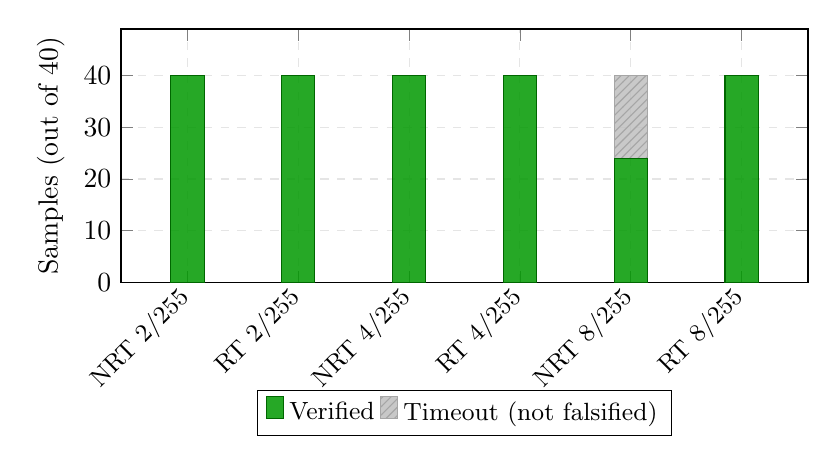
\begin{tikzpicture}
\begin{axis}[
    ybar stacked,
    width=0.85\columnwidth,
    height=4.8cm,
    bar width=12pt,
    ymin=0, ymax=49,
    ylabel={Samples (out of 40)},
    symbolic x coords={NRT $2/255$, RT $2/255$, NRT $4/255$, RT $4/255$, NRT $8/255$, RT $8/255$},
    xtick=data,
    x tick label style={font=\small, rotate=45, anchor=east, yshift=-2.5pt},
    legend style={at={(0.5,-0.425)}, anchor=north, font=\small, legend columns=2},
    grid=major,
    grid style={dashed, gray!20},
    ytick={0,10,20,30,40},
    enlarge x limits=0.12,
    every axis plot/.append style={fill opacity=0.85},
]
\addplot[fill=green!60!black, draw=green!40!black] coordinates 
    {(NRT $2/255$,40) (RT $2/255$,40) (NRT $4/255$,40) (RT $4/255$,40) (NRT $8/255$,24) (RT $8/255$,40)};
\addplot[fill=gray!50, draw=gray!70, postaction={pattern=north east lines, pattern color=gray!70}] coordinates
    {(NRT $2/255$,0) (RT $2/255$,0) (NRT $4/255$,0) (RT $4/255$,0) (NRT $8/255$,16) (RT $8/255$,0)};
\legend{Verified, Timeout (not falsified)}
\end{axis}
\end{tikzpicture}
\caption{Router formal verification (40 samples per configuration: 20 MNIST + 20 CIFAR-10, averaged over 5 runs). Both routers achieve 100\% RoCRA at practical $\varepsilon \leq 4/255$. At $\varepsilon = 8/255$, only NRT degrades -- and exclusively due to verification timeouts, not falsifications. Zero counterexamples were found in any configuration.}
\label{tab:router-verification}
\end{figure}

RoCRA ($\approx 100\%$) substantially exceeds end-to-end AA ($\approx 35\%$). This is expected: RoCRA verifies only the property $\arg\max_i \mathcal{G}_i(x') = m^*$ (correct expert selection) on individual samples, while AA measures end-to-end classification on the mixed test set where expert misclassifications dominate. The router achieves 100\% gating accuracy under PGD, but the selected expert may misclassify, reducing end-to-end AA. See Appendix~\ref{app:gap} for detailed analysis. \BW{If its important it should be in the main body.}

\textbf{Expert verification.}
We verified CIFAR-10 and MNIST experts (20 samples each, averaged over 5 runs) using ONNX models with BatchNorm folding and $\alpha$--$\beta$-CROWN with Gurobi. Figure~\ref{fig:expert-heatmap} summarizes ExCRA across both datasets, training paradigms, and perturbation budgets, revealing two key patterns. First, domain complexity dominates verifiability: MNIST-RT achieves 100\%/99\%/95\% ExCRA at $\varepsilon = \frac{2}{255}, \frac{4}{255}, \frac{8}{255}$ respectively, while CIFAR-10-NRT is completely unverifiable (ExCRA $= 0\%$) at all $\varepsilon$ levels. Second, robust training is a prerequisite for verification: CIFAR-10-RT achieves 90\% ExCRA at $\varepsilon = 2/255$ compared to 0\% for NRT, confirming that adversarial training smooths decision boundaries and tightens CROWN bounds. No falsifications occurred -- all failures are timeouts, not property violations.

\begin{figure}[t]
\centering
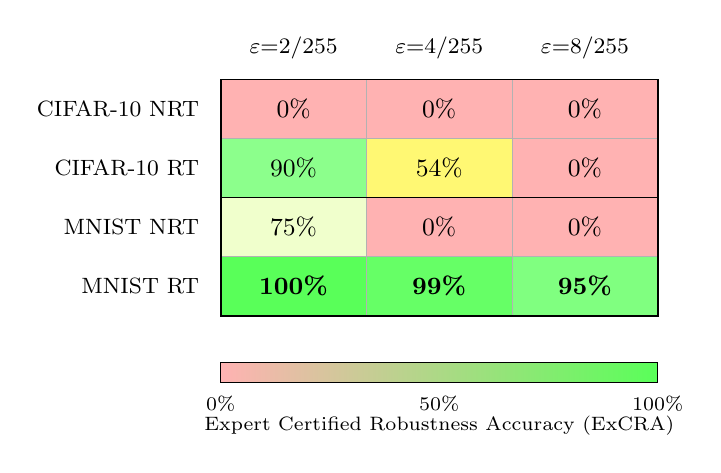
\begin{tikzpicture}[
    cell/.style={minimum width=1.85cm, minimum height=0.75cm, align=center,
                 font=\small, inner sep=0pt, outer sep=0pt},
]
% Column headers
\node[font=\footnotesize\bfseries] at (1.85*0.5, 0.4) {$\varepsilon{=}2/255$};
\node[font=\footnotesize\bfseries] at (1.85*1.5, 0.4) {$\varepsilon{=}4/255$};
\node[font=\footnotesize\bfseries] at (1.85*2.5, 0.4) {$\varepsilon{=}8/255$};

% Row headers
\node[font=\footnotesize, anchor=east] at (-0.15, -0.375) {CIFAR-10 NRT};
\node[font=\footnotesize, anchor=east] at (-0.15, -1.125) {CIFAR-10 RT};
\node[font=\footnotesize, anchor=east] at (-0.15, -1.875) {MNIST NRT};
\node[font=\footnotesize, anchor=east] at (-0.15, -2.625) {MNIST RT};

% --- Row 1: CIFAR-10 NRT (all 0%) ---
\fill[red!30] (0,0) rectangle (1.85,-0.75);
\fill[red!30] (1.85,0) rectangle (3.7,-0.75);
\fill[red!30] (3.7,0) rectangle (5.55,-0.75);
\node[cell] at (1.85*0.5, -0.375) {0\%};
\node[cell] at (1.85*1.5, -0.375) {0\%};
\node[cell] at (1.85*2.5, -0.375) {0\%};

% --- Row 2: CIFAR-10 RT ---
\fill[green!45] (0,-0.75) rectangle (1.85,-1.5);
\fill[yellow!55] (1.85,-0.75) rectangle (3.7,-1.5);
\fill[red!30] (3.7,-0.75) rectangle (5.55,-1.5);
\node[cell] at (1.85*0.5, -1.125) {90\%};
\node[cell] at (1.85*1.5, -1.125) {54\%};
\node[cell] at (1.85*2.5, -1.125) {0\%};

% --- Row 3: MNIST NRT ---
\fill[green!30!yellow!20] (0,-1.5) rectangle (1.85,-2.25);
\fill[red!30] (1.85,-1.5) rectangle (3.7,-2.25);
\fill[red!30] (3.7,-1.5) rectangle (5.55,-2.25);
\node[cell] at (1.85*0.5, -1.875) {75\%};
\node[cell] at (1.85*1.5, -1.875) {0\%};
\node[cell] at (1.85*2.5, -1.875) {0\%};

% --- Row 4: MNIST RT ---
\fill[green!65] (0,-2.25) rectangle (1.85,-3.0);
\fill[green!60] (1.85,-2.25) rectangle (3.7,-3.0);
\fill[green!50] (3.7,-2.25) rectangle (5.55,-3.0);
\node[cell] at (1.85*0.5, -2.625) {\textbf{100\%}};
\node[cell] at (1.85*1.5, -2.625) {\textbf{99\%}};
\node[cell] at (1.85*2.5, -2.625) {\textbf{95\%}};

% Grid lines
\draw[thin, gray!60] (0,0) grid[xstep=1.85, ystep=0.75] (5.55,-3.0);
\draw[semithick] (0,0) rectangle (5.55,-3.0);
% Horizontal separator between CIFAR-10 and MNIST blocks
\draw[semithick] (0,-1.5) -- (5.55,-1.5);

% Colorbar
\shade[left color=red!30, right color=green!65] (0,-3.6) rectangle (5.55,-3.85);
\draw[thin] (0,-3.6) rectangle (5.55,-3.85);
\node[font=\scriptsize, anchor=north] at (0,-3.9) {0\%};
\node[font=\scriptsize, anchor=north] at (2.775,-3.9) {50\%};
\node[font=\scriptsize, anchor=north] at (5.55,-3.9) {100\%};
\node[font=\scriptsize, anchor=north] at (2.775,-4.15) {Expert Certified Robustness Accuracy (ExCRA)};
\end{tikzpicture}
\caption{ExCRA across domains, training paradigms, and perturbation budgets (20 samples per configuration, mean over 5 runs). Green indicates high ExCRA; red indicates verification failure (timeout). Robust training (RT) is a prerequisite for verifiability: CIFAR-10 NRT is completely unverifiable at all $\varepsilon$, while MNIST RT maintains $\geq$95\% ExCRA even at $\varepsilon = 8/255$. Zero falsifications occurred in any configuration.}
\label{fig:expert-heatmap}
\end{figure}

\subsection{Empirical Adversarial Robustness}
\label{sec:eval-empirical}

We employed the Adversarial Robustness Toolbox (ART) with PGD attacks ($\varepsilon{=}8/255$, 7 iterations, step $2/255$) on $32{\times}32$ images from CIFAR-10 and MNIST.

\textbf{Individual expert robustness.}
Figure~\ref{fig:expert-robustness} confirms the expected robustness--accuracy tradeoff: CIFAR-10 incurs a 6.21\% clean accuracy cost for a 17.23\% adversarial accuracy gain; MNIST incurs only 0.02\% clean cost for a 44.71\% adversarial accuracy gain.

\begin{figure}[t]
\centering
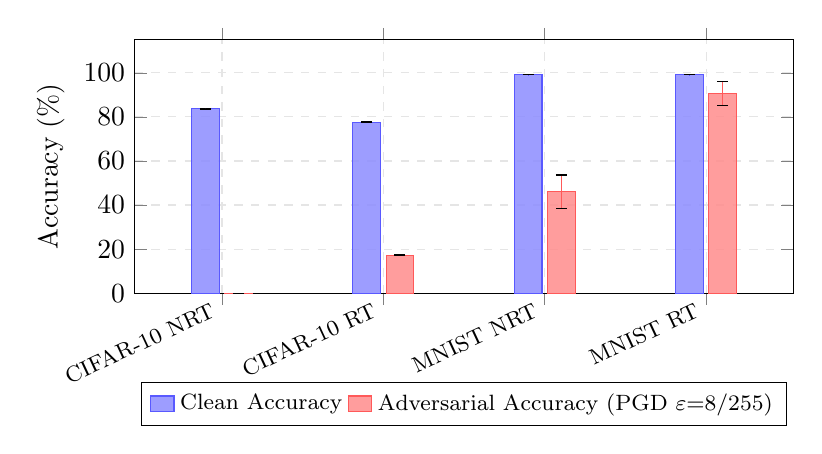
\begin{tikzpicture}
\begin{axis}[
    ybar,
    width=0.82\columnwidth,
    height=4.8cm,
    bar width=10pt,
    ymin=0, ymax=115,
    ylabel={Accuracy (\%)},
    symbolic x coords={CIFAR-10 NRT, CIFAR-10 RT, MNIST NRT, MNIST RT},
    xtick=data,
    x tick label style={font=\footnotesize, rotate=25, anchor=east},
    legend style={at={(0.5,-0.35)}, anchor=north, font=\footnotesize, legend columns=2},
    legend image code/.code={\fill[#1] (0cm,-0.1cm) rectangle (0.3cm,0.1cm);},
    grid=major,
    grid style={dashed, gray!20},
    ytick={0,20,40,60,80,100},
    enlarge x limits=0.18,
    every axis plot/.append style={fill opacity=0.85},
    clip=false,
]
% Clean Accuracy
\addplot[fill=blue!45, draw=blue!65,
    error bars/.cd, y dir=both, y explicit, error bar style={thin}
] coordinates {
    (CIFAR-10 NRT, 83.75) +- (0,0.21)
    (CIFAR-10 RT, 77.54) +- (0,0.26)
    (MNIST NRT, 99.19) +- (0,0.06)
    (MNIST RT, 99.17) +- (0,0.03)
};
% Adversarial Accuracy
\addplot[fill=red!45, draw=red!65,
    error bars/.cd, y dir=both, y explicit, error bar style={thin}
] coordinates {
    (CIFAR-10 NRT, 0.01) +- (0,0.01)
    (CIFAR-10 RT, 17.24) +- (0,0.27)
    (MNIST NRT, 46.06) +- (0,7.58)
    (MNIST RT, 90.77) +- (0,5.44)
};
\legend{Clean Accuracy, Adversarial Accuracy (PGD $\varepsilon{=}8/255$)}
\end{axis}
\end{tikzpicture}
\caption{Expert robustness--accuracy tradeoff (VerifiableCNN, mean $\pm$ std over 5 runs). The gap between blue (clean) and red (adversarial) bars represents the robustness gap. RT narrows the gap substantially for both domains, with MNIST achieving near-parity ($8.39\%$ gap) while CIFAR-10 retains a large gap ($60.30\%$), reflecting domain complexity.}
\label{fig:expert-robustness}
\end{figure}

\textbf{\textsf{MetaMoE} compositional robustness.}
We tested all 8 combinations of router training (RT/NRT) and expert configurations (4 combinations), each trained 5 times (40 total runs, 50 epochs router training). Table~\ref{tab:expert-impact} \BW{where is Table 1?} reveals that expert configuration dominates system robustness: the 13.15\% AA difference between Both-RT and Both-NRT far exceeds the $< 0.1\%$ router training effect. All 40 runs achieve 100\% gating accuracy under both clean and adversarial conditions, validating the invariance condition of Theorem~\ref{thm:compositional} and confirming that the router acts as a transparent switch. The weakest expert constrains system robustness, confirming modular robustness propagation. NRT router training is 3.2$\times$ faster with identical accuracy, yielding computational savings when routing is inherently stable.

\begin{table}[t]
\centering
\caption{Expert configuration dominates system robustness. Rows show expert training combinations averaged across both RT and NRT router training (which differ by $< 0.1\%$). 40 total runs: 8 configurations $\times$ 5 runs. All configurations achieve 100\% gating accuracy.}
\label{tab:expert-impact}
\small
\begin{tabular}{llll}
\toprule
\textbf{Expert Configuration} & \textbf{Clean Acc (\%)} & \textbf{Adv Acc (\%)} & \textbf{Robustness Gap} \\
\midrule
Both RT & $87.98 \pm 0.06$ & $41.93 \pm 0.41$ & $46.05\%$ \\
CIFAR10-NRT + MNIST-RT & $91.26 \pm 0.05$ & $37.66 \pm 0.66$ & $53.60\%$ \\
CIFAR10-RT + MNIST-NRT & $88.10 \pm 0.06$ & $33.56 \pm 0.90$ & $54.54\%$ \\
Both NRT & $91.32 \pm 0.06$ & $28.78 \pm 0.59$ & $62.54\%$ \\
\midrule
\multicolumn{4}{l}{\textit{Expert effect:} $\Delta_{\text{adv}} = 13.15\%$ (Both RT vs Both NRT)} \\
\multicolumn{4}{l}{\textit{Router effect:} $\Delta_{\text{adv}} < 0.1\%$ (RT Router vs NRT Router, 3.2$\times$ slower)} \\
\bottomrule
\end{tabular}
\end{table}

As detailed in Appendix~\ref{app:similarity}, GTSRB+PTSD (visually similar traffic sign datasets) achieves only 93.17\% gating accuracy and 29.47\% AA, compared to 100\% and 41.93\% for CIFAR10+MNIST (Both RT). The 12.12\% AA gap demonstrates that routing difficulty directly propagates to system robustness. Clean accuracy standard deviations range from 0.04\% to 0.08\%, indicating highly reproducible training outcomes. \BW{I think you need a clearer section where you describe what all the tests you are running are, describe the image sets, describe what happens to each image and to the collection of images as a whole. Describe how each metric is calculated (whether per image or for the group).}

\subsection{Empirical--Formal Correlation \BW{Rename empirical-formal}}
\label{sec:eval-correlation}

Figure~\ref{fig:gap-analysis} compares expert AA (PGD, $\varepsilon = 8/255$) with ExCRA ($\alpha$--$\beta$-CROWN, $\varepsilon = 2/255$). Because the perturbation budgets differ, absolute values are not directly comparable; we focus on whether the model ranking by AA predicts the ranking by ExCRA. Within each domain, higher AA monotonically associates with higher ExCRA: MNIST NRT$\to$RT increases both AA ($46\% \to 91\%$) and ExCRA ($75\% \to 100\%$); CIFAR-10 NRT$\to$RT moves from completely unverifiable (ExCRA $= 0\%$) to ExCRA $= 90\%$. Routers are excluded from this comparison because RoCRA verifies routing invariance (a per-sample argmax property) while router AA measures end-to-end classification, making their comparison uninformative (see Section~\ref{sec:eval-formal}).

\begin{figure}[t]
\centering
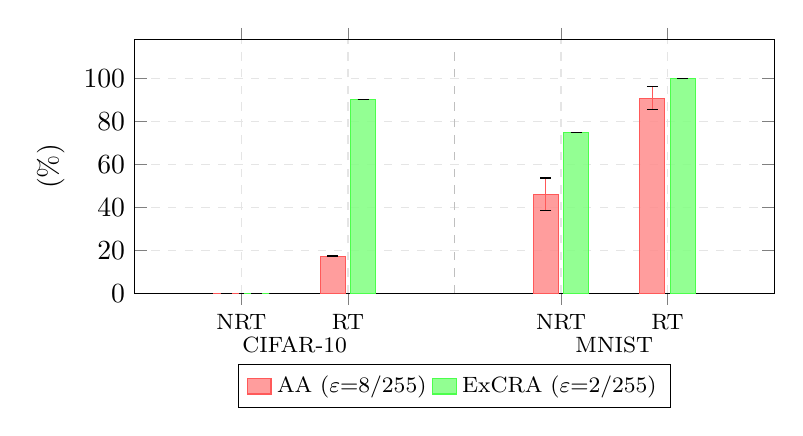
\begin{tikzpicture}
\begin{axis}[
    ybar,
    width=0.80\columnwidth,
    height=4.8cm,
    bar width=9pt,
    ymin=0, ymax=118,
    ylabel={(\%)},
    xtick={1,2, 4,5},
    xticklabels={NRT, RT, NRT, RT},
    x tick label style={font=\footnotesize},
    xmin=0, xmax=6,
    legend style={at={(0.5,-0.28)}, anchor=north, font=\footnotesize, legend columns=2},
    legend image code/.code={\fill[#1] (0cm,-0.1cm) rectangle (0.3cm,0.1cm);},
    grid=major,
    grid style={dashed, gray!20},
    ytick={0,20,40,60,80,100},
    every axis plot/.append style={fill opacity=0.85},
    clip=false,
]
% Adversarial Accuracy (AA)
\addplot[fill=red!45, draw=red!65,
    error bars/.cd, y dir=both, y explicit, error bar style={thin}
] coordinates {
    (1, 0.01) +- (0,0.01)
    (2, 17.24) +- (0,0.27)
    (4, 46.06) +- (0,7.58)
    (5, 90.77) +- (0,5.44)
};
% Expert Certified Robustness Accuracy (ExCRA)
\addplot[fill=green!50, draw=green!70,
    error bars/.cd, y dir=both, y explicit, error bar style={thin}
] coordinates {
    (1, 0.0) +- (0,0.0)
    (2, 90.0) +- (0,0.0)
    (4, 75.0) +- (0,0.0)
    (5, 100.0) +- (0,0.0)
};
% Gap annotations (Delta) above bar pairs
% \node[font=\scriptsize, text=black!70] at (axis cs:1, 8) {--};
% \node[font=\scriptsize, text=black!70] at (axis cs:2, 98) {$\Delta{=}73$};
% \node[font=\scriptsize, text=black!70] at (axis cs:4, 83) {$\Delta{=}29$};
% \node[font=\scriptsize, text=black!70] at (axis cs:5, 108) {$\Delta{=}9$};
% Separator line between groups
\draw[thin, dashed, gray!50] (axis cs:3, 0) -- (axis cs:3, 115);
% Group labels below tick labels
\node[font=\footnotesize, text=black] at (axis cs:1.5, -24) {CIFAR-10};
\node[font=\footnotesize, text=black] at (axis cs:4.5, -24) {MNIST};
\legend{AA ($\varepsilon{=}8/255$), ExCRA ($\varepsilon{=}2/255$)}
\end{axis}
\end{tikzpicture}
\caption{Expert empirical--formal robustness correlation (AA at $\varepsilon = 8/255$, ExCRA at $\varepsilon = 2/255$; mean $\pm$ std over 5 runs). AA is an empirical heuristic (PGD attack, no formal guarantee); ExCRA is a formal metric (sound verifier proof). Because the perturbation budgets differ, absolute values are not directly comparable; the key observation is that within each domain, the model ranking by AA predicts the ranking by ExCRA. CIFAR-10 NRT is completely unverifiable (both metrics $\approx 0\%$). Router results are omitted because RoCRA (routing invariance) and router AA (end-to-end classification) measure different properties; see Section~\ref{sec:eval-formal}.}
\label{fig:gap-analysis}
\end{figure}

The practical implication is clear: robust training of experts is mandatory for verifiability. CIFAR-10-NRT is completely unverifiable (ExCRA $= 0\%$), while within RT models, higher empirical robustness correlates with higher formal certification in our study.

\subsection{Scalability}
\label{sec:eval-scalability}

\textbf{Training time.}
We compared \textsf{MetaMoE} against monolithic training when incrementally adding a third dataset (MNIST) to an existing 2-dataset system (GTSRB + CIFAR-10). The monolithic approach must retrain on all three datasets from scratch (151 mins), while \textsf{MetaMoE} only trains a new expert (72.5 mins) and fine-tunes the frozen router (30 mins), yielding a 16.7\% end-to-end speedup (202 vs.\ 242.5 total mins). This gap widens as more experts are added, since per-expert cost is fixed while monolithic retraining grows with dataset count. See Appendix~\ref{app:training-time} for the full breakdown \BW{bring timings into main body of the paper.}.

\textbf{Inference scaling.}
Inference latency follows $L(k) = L_{\text{router}} + \sum_{i=1}^k L_{\text{expert}_i}$, where $L_{\text{router}}$ is constant and each expert contributes $\sim$40--50ms. Figure~\ref{tab:inference} confirms $O(k)$ scaling: at fixed $k{=}1$, latency remains $\sim$71ms regardless of whether the system contains 2 or 5 total experts.

\begin{figure}[t]
\centering
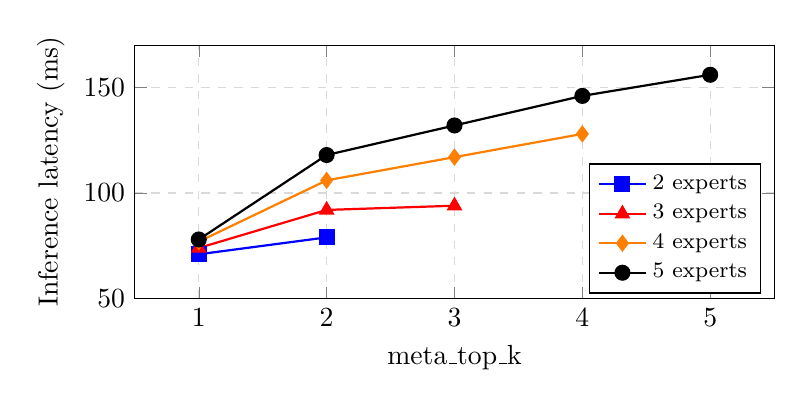
\begin{tikzpicture}
\begin{axis}[
    width=0.80\columnwidth,
    height=4.8cm,
    xlabel={meta\_top\_k},
    ylabel={Inference latency (ms)},
    xmin=0.5, xmax=5.5,
    ymin=50, ymax=170,
    xtick={1,2,3,4,5},
    legend style={at={(0.98,0.02)}, anchor=south east, font=\footnotesize},
    grid=major,
    grid style={dashed, gray!30},
    every axis plot/.append style={thick, mark size=2.5pt},
]
\addplot[color=blue, mark=square*] coordinates {(1,71) (2,79)};
\addlegendentry{2 experts}
\addplot[color=red, mark=triangle*] coordinates {(1,74) (2,92) (3,94)};
\addlegendentry{3 experts}
\addplot[color=orange, mark=diamond*] coordinates {(1,77) (2,106) (3,117) (4,128)};
\addlegendentry{4 experts}
\addplot[color=black, mark=*] coordinates {(1,78) (2,118) (3,132) (4,146) (5,156)};
\addlegendentry{5 experts}
\end{axis}
\end{tikzpicture}
\caption{Inference latency (ms) vs.\ meta\_top\_k for different numbers of total experts.}
\label{tab:inference}
\end{figure}

\textbf{Verification scaling.}
The compositional verification advantage grows linearly with $N$: our $N{=}2$ setting yields a ${\sim}$2.4$\times$ verification cost reduction, scaling to ${\sim}$7$\times$ at $N{=}7$ datasets (Table~\ref{tab:notation}), since monolithic cost scales with total system size while per-component cost remains fixed. \BW{where is Table 3? Is there a Table 2? should be in the main body I think.}

\textbf{Why monolithic MoE verification is infeasible.}

Compositional verification is not merely more efficient -- it is currently the \emph{only} viable approach, due to two independent structural barriers. First, ONNX export is trace-based~\cite{pytorchonnx}: the exporter records a single execution path, hard-coding the router's expert selection for the dummy input into a static graph~\cite{pytorchcontrolflow}. The ONNX IR is fundamentally a static, side-effect-free computation graph~\cite{onnxir}; its \texttt{If} operator requires identically shaped branch outputs~\cite{pytorchcontrolflow}, which is incompatible with experts having different class space dimensions. Second, all current verifiers operate on fixed computational graphs. Bound propagation (CROWN~\cite{xu2020abcrown}, $\alpha$--$\beta$-CROWN~\cite{wang2021}) is undefined when graph topology varies per input; SMT-based (Marabou~\cite{katz2022marabou}) and abstract-interpretation (ERAN~\cite{singh2019eran}) verifiers likewise require fixed topologies. No VNN-COMP benchmark (2021--2025) has included models with input-dependent routing~\cite{kaulen2025}. Our compositional decomposition sidesteps both barriers by reducing the problem to standard feedforward CNN verification, yielding $O(1)$ per-component cost and compatibility with all existing monolithic verifiers.


\subsection{Limitations}
\label{sec:limitations}

Theorem~\ref{thm:compositional} establishes a biconditional for hard routing ($k{=}1$) with disjoint expert class spaces. Extending the result to soft or top-$k$ routing requires verifying invariance of the full top-$k$ set and stability of the routing weights, since a small perturbation could reorder activated experts even when no single logit crosses a decision boundary. For overlapping class spaces, only the sufficient direction holds (Section~\ref{sec:compositional}), weakening the compositional guarantee to a one-sided implication.

Our experiments use small verification-compatible CNNs (${\sim}$96K parameters per expert, ${\sim}$38K for the router). The compositional decomposition reduces the verification target, yet verifying a single large expert remains an open challenge -- $\alpha$--$\beta$-CROWN and comparable tools face memory and time constraints well before production scale.

The framework also depends on the router's ability to discriminate between expert domains. For visually dissimilar datasets (CIFAR-10 vs.\ MNIST), the router achieves 100\% gating accuracy and Theorem~\ref{thm:compositional} applies directly. For visually similar datasets (GTSRB vs.\ PTSD), gating accuracy drops to 93.17\% (Appendix~\ref{app:similarity}), violating router invariance at ${\sim}$7\% of inputs.

We verified 20--40 samples per configuration at a cost of ${\sim}$11 seconds per router sample and up to 300 seconds per expert sample. While zero falsifications is encouraging, a larger verification budget would strengthen statistical confidence. We consider only $\ell_\infty$-bounded perturbations; other threat models ($\ell_2$, patch attacks) require separate verification specifications.

\section{Conclusion and Future Work}

We presented \textsf{MetaMoE}, a framework for compositional robustness verification of heterogeneous MoE systems. The central result is Theorem~\ref{thm:compositional}: for hard-routed MoE with disjoint expert class spaces, router invariance and expert robustness are individually necessary and jointly sufficient for system robustness. This decomposition reduces verification cost from the full system to the largest single component, with the advantage scaling linearly in the number of experts (${\sim}$2.4$\times$ at $N{=}2$, ${\sim}$7$\times$ at $N{=}7$). We validated the theorem both formally, via $\alpha$--$\beta$-CROWN, and empirically, via PGD attacks, across 8 MoE configurations and 40 training runs.

The experiments reveal that for dissimilar datasets, expert robustness dominates system behavior (13.15\% AA difference between all-RT and all-NRT experts) while the router training paradigm has negligible impact ($< 0.1\%$), allowing a 3.2$\times$ router training speedup by forgoing adversarial augmentation. Router verification achieves 100\% RoCRA at $\varepsilon \leq 4/255$ with zero falsifications across all 40 runs, satisfying the invariance condition of Theorem~\ref{thm:compositional}. Within each domain, higher AA monotonically associates with higher ExCRA, and non-robust training on complex domains yields complete verification failure (ExCRA $= 0\%$ for CIFAR-10-NRT), establishing robust training as a prerequisite for verifiability.

We see three directions for extending this work. First, generalizing Theorem~\ref{thm:compositional} to soft and top-$k$ routing will require reasoning about weight stability under perturbation; probabilistic verification methods~\cite{chwialkowski2025probabilistic} may offer relaxed but practical guarantees in that setting. Second, strengthening the empirical--formal correlation on complex domains calls for tighter bound propagation or certified training methods such as CROWN-IBP~\cite{zhang2020} integrated into the expert training pipeline. Third, the GTSRB+PTSD results (Appendix~\ref{app:similarity}) expose a richer problem than routing failure alone: when experts share semantically equivalent classes, a misroute may not cause a misclassification. Relaxing Theorem~\ref{thm:compositional} to account for cross-expert redundancy would yield a more permissive compositional guarantee for similar-domain systems. We hope the compositional perspective introduced here provides a useful foundation for building verifiable modular AI in safety-critical applications.

\bibliographystyle{splncs04}
\bibliography{references_saiv2026}

\appendix

\section{Training Hyperparameters}
\label{app:hyperparams}

\subsection{Expert Training Configuration}

All experts trained with Adam optimizer, learning rate $1 \times 10^{-3}$, Label Smoothing Cross Entropy (smoothing $= 0.1$), 200 epochs (early stopping), batch size 128, random flips and crops. RT: PGD with $\varepsilon = 8/255$, 7 iterations, step size $\alpha = 2/255$, $L_\infty$ norm.

\subsection{Router Training Configuration}

Adam optimizer, learning rate $1 \times 10^{-3}$, weight decay $5 \times 10^{-4}$, Cross Entropy loss, 50 epochs (early stopping), batch size 128. RT: same PGD configuration as experts.

\section{ONNX Export Details}
\label{app:onnx}

\subsection{BatchNorm Folding}

For a convolutional layer with weights $W \in \mathbb{R}^{C_{\text{out}} \times C_{\text{in}} \times k \times k}$ (where $C_{\text{out}}$ is the number of output channels, $C_{\text{in}}$ the number of input channels, and $k \times k$ the kernel size) and bias $b \in \mathbb{R}^{C_{\text{out}}}$, followed by a BatchNorm layer with running mean $\mu_i$, running variance $\sigma^2_i$, learnable scale $\gamma_i$, and shift $\beta_i$ (all per output channel~$i$), with numerical stability constant $\varepsilon_{\text{bn}} = 10^{-5}$, the folded (merged) parameters are:
\begin{align}
W'_{i,j,m,n} &= \gamma_i \cdot \frac{W_{i,j,m,n}}{\sqrt{\sigma^2_i + \varepsilon_{\text{bn}}}} \quad \forall i,j,m,n \\
b'_i &= \frac{\gamma_i}{\sqrt{\sigma^2_i + \varepsilon_{\text{bn}}}} \cdot (b_i - \mu_i) + \beta_i \quad \forall i
\end{align}
Here, the index $i$ ranges over output channels ($1 \leq i \leq C_{\text{out}}$), $j$ over input channels, and $m, n$ over spatial kernel dimensions. The folded layer $\text{Conv}(W', b')$ is mathematically equivalent to $\text{BatchNorm}(\text{Conv}(W, b))$, eliminating the BatchNorm operator from the ONNX graph.

Verification: $\max|f_{\text{original}}(x) - f_{\text{folded}}(x)| < 10^{-5}$ for random inputs. All models exported with PyTorch 2.0+, ONNX opset 13, static input shape $(1, 3, 32, 32)$, raw logits output.

\section{Dataset Characteristics}
\label{app:datasets}

\begin{table}[t]
\centering
\caption{Dataset statistics.}
\small
\begin{tabular}{lllll}
\toprule
\textbf{Dataset} & \textbf{Classes} & \textbf{Train} & \textbf{Test} & \textbf{Domain} \\
\midrule
CIFAR-10 & 10 & 50,000 & 10,000 & General objects \\
MNIST & 10 & 60,000 & 10,000 & Handwritten digits \\
GTSRB & 43 & 39,209 & 12,630 & German traffic signs \\
PTSD & 43 & 14,405 & 2,421 & Persian traffic signs \\
BTSD & 62 & 4,575 & 2,520 & Belgian traffic signs \\
ETSD & 55 & 6,133 & 2,027 & European traffic signs \\
TSRD & 58 & 4,170 & 1,994 & Chinese traffic signs \\
\bottomrule
\end{tabular}
\end{table}

\section{Dataset and Expert Notation}
\label{app:notation}

\begin{table}[t]
\centering
\caption{Dataset and expert notation. Each expert is trained in two paradigms: Non-Robust Training (NRT) and Robust Training (RT).}
\label{tab:notation}
\begin{tabular}{llll}
\toprule
\textbf{Dataset} & \textbf{Meta-class} & \multicolumn{2}{c}{\textbf{Notation}} \\
 & & \textbf{NRT} & \textbf{RT} \\
\midrule
CIFAR-10 & $E_0$ & $E_{0\_\text{CNN\_NRT}}$ & $E_{0\_\text{CNN\_RT}}$ \\
MNIST & $E_1$ & $E_{1\_\text{CNN\_NRT}}$ & $E_{1\_\text{CNN\_RT}}$ \\
GTSRB & $E_2$ & $E_{2\_\text{CNN\_NRT}}$ & $E_{2\_\text{CNN\_RT}}$ \\
PTSD & $E_3$ & $E_{3\_\text{CNN\_NRT}}$ & $E_{3\_\text{CNN\_RT}}$ \\
BTSD & $E_4$ & $E_{4\_\text{CNN\_NRT}}$ & $E_{4\_\text{CNN\_RT}}$ \\
ETSD & $E_5$ & $E_{5\_\text{CNN\_NRT}}$ & $E_{5\_\text{CNN\_RT}}$ \\
TSRD & $E_6$ & $E_{6\_\text{CNN\_NRT}}$ & $E_{6\_\text{CNN\_RT}}$ \\
\bottomrule
\end{tabular}
\end{table}

\section{Hardware and Software Environment}
\label{app:hardware}

Training/Inference: Intel Core i7-14700K (20 cores), NVIDIA GeForce RTX 4060 (8GB), 64GB DDR5, Ubuntu 22.04.5 LTS. Software: Python 3.10.12, PyTorch 2.1.0+cu121, CUDA 12.1, ONNX 1.15.0, $\alpha$--$\beta$-CROWN commit d4c79e3, Gurobi 11.0.0, ART 1.17.0. All experiments use fixed random seed 42.

\section{Detailed Architecture Specifications}
\label{app:architecture}

The VerifiableCNN architecture used for experts (${\sim}$96K parameters with BatchNorm, 43 classes; ${\sim}$94K for 10 classes) and router (${\sim}$38K parameters without BatchNorm):

\textbf{Convolutional Feature Extraction:}
Conv Block 1: Conv2d($3 \to 20$, $3 \times 3$, padding=1), ReLU, AvgPool($2 \times 2$) $\to 20 \times 16 \times 16$.
Conv Block 2: Conv2d($20 \to 28$, $3 \times 3$, padding=1), ReLU, AvgPool($2 \times 2$) $\to 28 \times 8 \times 8$.
Conv Block 3: Conv2d($28 \to 40$, $3 \times 3$, padding=1), ReLU, AvgPool($2 \times 2$) $\to 40 \times 4 \times 4$.
Conv Block 4: Conv2d($40 \to 56$, $3 \times 3$, padding=1), ReLU $\to 56 \times 4 \times 4$.

\textbf{Classification Head:} Flatten($56 \times 4 \times 4 = 896$), Linear($896 \to 64$), ReLU, Dropout($0.3$), Linear($64 \to C$) where $C = C_i$ for experts or $C = N$ for router. Output: raw logits (no softmax).

\textbf{Expert vs.\ Router:} Experts include BatchNorm after each convolution (${\sim}$96K params for 43 classes); the router omits BatchNorm for deterministic verification behavior (${\sim}$38K params for $N{=}2$).

\textbf{Design Rationale:} Gradual channel growth ($3 \to 20 \to 28 \to 40 \to 56$) compensates for narrow channels. Average pooling (linear operation) facilitates LP-based verification. Router omits BatchNorm to eliminate train/eval discrepancies. All $3 \times 3$ convolutions enable uniform bound propagation.

\section{Empirical--Formal Robustness Correlation Analysis}
\label{app:gap}

We evaluate AA using PGD attacks at $\varepsilon = 8/255$ (the training perturbation budget) and ExCRA using $\alpha$--$\beta$-CROWN at $\varepsilon = 2/255$ (a practical verification budget). Because these use different perturbation budgets, their absolute values cannot be compared directly -- at a fixed $\varepsilon$, formal verification is sound so $\text{ExCRA} \leq \text{AA}$ always holds. Instead, we examine whether models that rank higher by AA also rank higher by ExCRA. This correlation holds within each domain: for both CIFAR-10 and MNIST, RT models rank above NRT models on both metrics.

\textbf{Critical finding:} CIFAR-10-NRT exhibits ExCRA $= 0\%$ (complete verification failure), demonstrating robust training is a prerequisite for verifiability. Non-robust models produce excessively loose CROWN bounds due to chaotic decision boundaries.

\section{Training Time Breakdown}
\label{app:training-time}

Tables~\ref{tab:train-2ds} and~\ref{tab:train-3ds} show the full training time comparison between monolithic and \textsf{MetaMoE} compositional training.

\begin{table}[t]
\centering
\caption{Training time comparison (2 datasets: GTSRB + CIFAR-10).}
\label{tab:train-2ds}
\small
\begin{tabular}{@{}llp{4.2cm}@{}}
\toprule
 & \textbf{Monolithic} & \textbf{\textsf{MetaMoE} (2 experts)} \\
\midrule
Training time & 91.5 mins & 99.5 mins \\
Clean accuracy & 93.15\% & 92.80\% \\
Details & Combined training & GTSRB: 33.5 mins \newline CIFAR-10: 54 mins \newline Router: 15 mins \\
\bottomrule
\end{tabular}
\end{table}

\begin{table}[t]
\centering
\caption{Training time comparison (3 datasets: + MNIST, incremental addition).}
\label{tab:train-3ds}
\small
\begin{tabular}{@{}lp{3.8cm}p{3.8cm}@{}}
\toprule
 & \textbf{Monolithic} & \textbf{\textsf{MetaMoE} (3 experts)} \\
\midrule
Training time & 242.5 mins & 202.0 mins \\
Clean accuracy & 94.97\% & 93.61\% \\
Details & Initial 2-dataset: 91.5 mins \newline Retrain to add MNIST: 151 mins & Initial 2-expert MoE: 99.5 mins \newline Add MNIST expert: 72.5 mins \newline Fine-tune router: 30 mins \\
\bottomrule
\end{tabular}
\end{table}

The key insight is the incremental cost: adding a new dataset requires 151 mins of full retraining for the monolithic model vs.\ 102.5 mins (72.5 + 30) for \textsf{MetaMoE}. Of the \textsf{MetaMoE} cost, only the 30-min router fine-tuning step touches the existing system; the 72.5-min expert training is fully independent and parallelizable.

\section{Dataset Similarity Analysis: GTSRB+PTSD vs.\ CIFAR10+MNIST}
\label{app:similarity}

GTSRB+PTSD (both traffic sign datasets) achieves only 93.17\% gating accuracy vs.\ 100\% for CIFAR10+MNIST. The 6.83\% routing error exceeds the margin explained by expert imbalance, indicating inherent domain confusion from shared visual structures.

Adversarial robustness gap: GTSRB+PTSD achieves 29.47\% AA vs.\ 41.59\% for CIFAR10+MNIST (12.12\% gap). Adversarial attacks exploit routing uncertainty more effectively when the router must distinguish between visually similar domains.

The compositional verification property (Verified router $\land$ Verified expert $\implies$ Verified system) holds trivially for dissimilar datasets (100\% gating accuracy) but requires additional verification effort for similar domains, where probabilistic guarantees may be needed.

\end{document}
